\documentclass{article}
% translate with >> pdflatex -shell-escape <file>

% This file is an extract of the PGFPLOTS manual, copyright by Christian Feuersaenger.
% 
% Feel free to use it as long as you cite the pgfplots manual properly.
%
% See
%   http://pgfplots.sourceforge.net/pgfplots.pdf
% for the complete manual.
%
% Any required input files (for <plot table> or <plot file> or the table package) can be downloaded
% at
% http://www.ctan.org/tex-archive/graphics/pgf/contrib/pgfplots/doc/latex/
% and
% http://www.ctan.org/tex-archive/graphics/pgf/contrib/pgfplots/doc/latex/plotdata/

\usepackage{pgfplots}
\pgfplotsset{compat=newest}

\pagestyle{empty}

\begin{document}
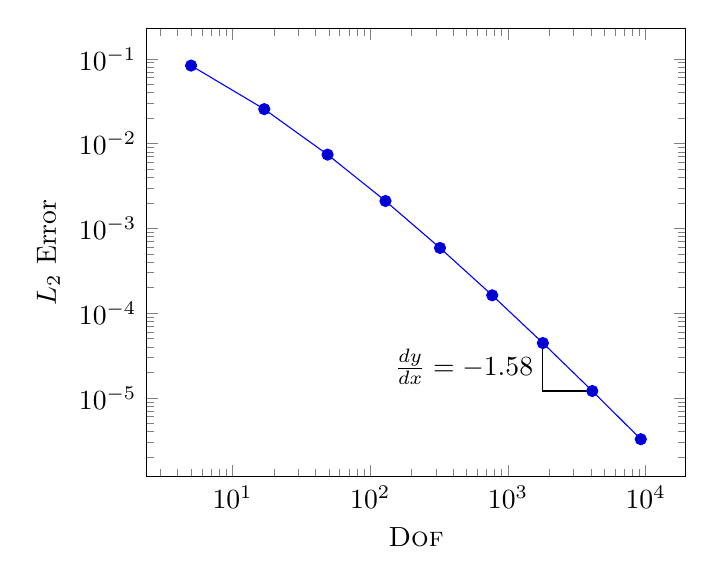
\begin{tikzpicture}
\begin{loglogaxis}[
	xlabel=\textsc{Dof},
	ylabel=$L_2$ Error
]
\draw 
		(axis cs:1793,4.442e-05)
	|-  (axis cs:4097,1.207e-05)
	node[near start,left] 
	{$\frac{dy}{dx} = -1.58$};

\addplot coordinates {
	(5,    8.312e-02)
	(17,   2.547e-02)
	(49,   7.407e-03)
	(129,  2.102e-03)
	(321,  5.874e-04)
	(769,  1.623e-04)
	(1793, 4.442e-05)
	(4097, 1.207e-05)
	(9217, 3.261e-06)
};
\end{loglogaxis}
\end{tikzpicture}
\end{document}
